\flushleft
\begin{minipage}{.75\textwidth}
\begin{Exercise}[label = wdsstrecke, title = Widerstandsstrecke, difficulty = 3, origin = IPhO 1996 ]
Bestimme den Widerstand zwischen den Punkten $A$ und $B$
	\end{Exercise}
\end{minipage}
\hfill
\begin{minipage}{.2\textwidth}
	\centering
	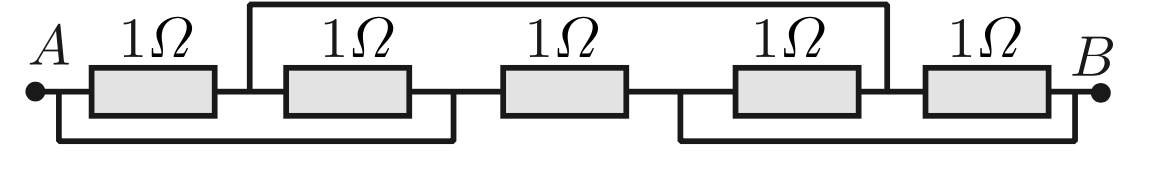
\includegraphics[scale = .2]{../tasks/ipho/wdsstrecke.png}
\end{minipage}
\begin{Answer}[ref = wdsstrecke]
	Um die Aufgabe einfach lösen zu können, muss man wissen, dass wen zwei Punkte nur durch einen Draht verbunden sind, sie auf dem gleichen Potential liegen müssen. Das liegt einfach daran, dass über ihnen keine Spannung abfallen kann, weil nichts da ist, an dem Spannung abfallen könnte \footnote{Außer natürlich der Draht selber. Aber in fast allen Aufgaben geht man davon aus, dass Drähte widerstandsfrei sind. Wenn das nicht so ist, sollte es auch angegeben sein.}
\end{Answer}